\section{GenSim}

\subsection{The GenSim ADL}

\begin{frame}{The GenSim ADL}

\end{frame}

\begin{frame}{The GenSim ADL}

GenSim is the name of our ADL toolset. It is designed to:

\begin{itemize}
	\item ... be intuitive and easy to learn
	\item ... create high performance simulation tools
	\item ... be extensible in terms of analyses

\end{itemize}

\end{frame}

\begin{frame}{GenSim Toolflow}

\centering
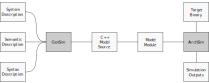
\includegraphics[width=\textwidth]{figures/gensim-toolflow}

\end{frame}

\begin{frame}{GenSim Model Components}

A GenSim description consists of several components
\begin{itemize}
\pause
\item A `System' component
\begin{itemize}
\item Available instruction sets
\item Register file layout
\item Configurable Features
\end{itemize}
\pause
\item A `Syntax' component
\begin{itemize}
\item Instruction formats
\item Instruction encoding
\end{itemize}
\pause
\item A `Semantics' component
\begin{itemize}
\item Instruction behaviours
\item Exception behaviour
\end{itemize}

\end{itemize}

\end{frame}
